\documentclass{article}
\usepackage[a4paper, total={5.8in, 10in}]{geometry}
\usepackage{graphicx}
\usepackage[T1]{fontenc}
\usepackage{tgpagella}
\usepackage{amsthm, amssymb, amsmath, amsfonts, bm}
% \usepackage{subcaption} % Include this in your preamble
% \usepackage[caption=false]{subfig} % To manage captions in minipage

\usepackage[colorlinks=true, linkcolor=blue, urlcolor=blue, citecolor=blue, filecolor=blue]{hyperref}

% \newtheorem*{corollary*}{Corollary}
% \newtheorem*{theorem*}{Theorem}
% \newtheorem*{remark*}{Remark}

\title{Arithmetic Asian Options}
\author{Ji Won Ahn}
\date{}

\newtheorem{question}{Question}
\newtheorem{qpart}{Part}[question]
\newtheorem*{solution}{Solution}

\newcommand{\R}{\mathbb{R}}
\newcommand{\N}{\mathbb{N}}
\newcommand{\set}[2]{ \{ #1\ |\ #2 \} }

\usepackage[style=numeric,sorting=none]{biblatex}
\addbibresource{refs.bib}

\begin{document}

\maketitle

\section{Introduction}

The Asian option is a path-dependent exotic option whose payoff involves a historical average price of the underlying asset, first successfully priced in 1987 by Mark Standish and David Spaughton of Bankers Trust during their business stay in Japan.
Due to the averaging mechanism, Asian options have lower volatility and offers greater protection against price fluctuations compared to the plain European counterparts and are prevalent in the commodities, currency and energy markets.
We begin with the geometric Brownian motion (GBM) stock process, \(S(t)\) whose dynamics are given by
\begin{equation}
    d S(t)=r S(t) d t+\sigma S(t) d \widetilde{W}(t),\quad r, \sigma > 0;\label{eq:1}
\end{equation}
where \(\widetilde{W}(t), 0\leq t\leq T\) denotes the Brownian motion under the risk neutral measure \(\widetilde{\mathbb{P}}\).
The payoff of the Asian call with the non-negative fixed-strike \(K\) under arithmetic averaging at time \(T\) is given by
\begin{equation}
    V(T) = \left(\frac{1}{T} \int_0^T S(t) d t-K\right)^{+}. \label{eq:2}
\end{equation}
Assuming a constant interest rate \(r\), the price for \(t \leq T\) is given by the risk-neutral pricing formula
\begin{equation}
    V(t)=\tilde{\mathbb{E}}\left[e^{-r(T-t)} V(T) \mid \mathcal{F}(t)\right], \quad 0 \leq t \leq T. \label{eq:3}
\end{equation}
However, the formula does not admit a closed form solution due to the fact that the arithmetic average is not log-normally distributed.
As such, the option prices often rely on numerical techniques or approximation methods.
This expository paper aims to outline the general theory of pricing the arithmetic fixed-strike Asian option along with some numerical implementations used for valuation.


\section{Valuation Problem for Asian Options}
\newcommand{\F}{\mathcal{F}}
\newcommand{\tP}{\widetilde{\mathbb{P}}}
\newcommand{\tW}{\widetilde{W}(t)}
\newcommand{\E}{\mathbb{E}}
\newcommand{\tE}{\widetilde{\E}}

\label{Valuation Problem for Asian Options}

Let \((\Omega, \F, (\F(t))_{t \geq 0}, \tP)\) be the filtered probability space with risk-neutral measure \(\tP\) with the given filtration \((\F(t))_{t \geq 0}\) generated by the Brownian motion \(\tW\).
Defining \(Y(t) = \int_0^t S(t) dt\), the payoff at time \(T\) is given by
\begin{equation}
    V(T) = \left( \frac{1}{T} Y(T) - K\right)^+. 
\end{equation}
The risk-neutral pricing formula in equation \eqref{eq:3} cannot invoke the Markov property with $t$ and $S(t)$.
However, \(S(t)\) is a solution to equation \eqref{eq:1} and $Y(t)$ is a solution to $dY(t) = S(t) dt$ with $Y(0) = 0$, so the two-dimensional process $(S(t), Y(t))$ is a Markov process.
Hence, now the risk-neutral pricing formula in equation \eqref{eq:3} may now invoke the Markov property, where the price is given by a function $v(t, x, y)$ such that
\begin{equation}
    v(t, S(t), Y(t))=\tE\left[e^{-r(T-t)} V(T) \mid \mathcal{F}(t)\right], \quad 0 \leq t \leq T. \label{eq:5}
\end{equation}
Since equation \eqref{eq:5} shows that the discounted option price \(e^{-rt}v(t, S(t), Y(t))\) is a \(\tP\)-martingale, we apply Itò's formula to the discounted option process and see that drift term has to equate to zero. In particular, the price is shown to satisfy the Asian call option PDE \cite{shreve2004stochastic}
\begin{equation}
    r v(t, x, y) = v_t(t, x, y) + r x v_x(t, x, y) + x v_y(t, x, y) + \frac{\sigma^2 x^2}{2} v_{xx}(t, x, y), \label{eq:6}
\end{equation}
where $0<t\leq T, \enspace x \geq 0, \enspace y \in \mathbb{R}$ and boundary conditions
\begin{align*}
    v(t, 0, y) & =e^{-r(T-t)}\left(\frac{y}{T}-K\right)^{+}, 0 \leq t<T, y \in \mathbb{R}, \\
\lim _{y \downarrow-\infty} v(t, x, y) & =0,0 \leq t<T, x \geq 0, \\
v(T, x, y) & =\left(\frac{y}{T}-K\right)^{+}, x \geq 0, y \in \mathbb{R}.
\end{align*}
A short position in the Asian call is hedged by equating \(d(e^{-rt}X(t)) = d(e^{-rt} v(t, S(t), Y(t)))\). This obtains the amount of the underlying asset to hold, $\Delta(t)$, i.e. the delta-hedging formula
\begin{equation*}
    \Delta(t) = v_x(t, S(t), Y(t)).
\end{equation*}
Alternatively, Shreve prices an Asian call that may be averaged a smaller time frame $c \leq T$, with the payoff
\begin{equation*}
    V(T) = \left(\frac{1}{c} \int_{T-c}^{T} S(t) \, dt - K\right)^+,\quad 0 < c \leq T.
\end{equation*}
Firstly, he creates a portfolio process $X(t)$
that holds $\gamma(t)$ shares of the underlying, given by
\begin{equation*}
    \gamma(t) = 
\begin{cases} 
    \frac{1}{rc}(1 - e^{-rc}), & 0 \leq t \leq T - c, \\[8pt]
    \frac{1}{rc} \left(1 - e^{-r(T - t)}\right), & T - c \leq t \leq T,
\end{cases}        
\end{equation*}
and terminal condition $X(T) = \frac{1}{c}\int_{T-c}^T S(t)\ dt $.
Shreve \cite{shreve2004stochastic} derives $X(t)$ in its explicit form to be
\begin{align*}
    X(t) = \frac{1}{rc} \left(1 - e^{-r(T - t)}\right) S(t) 
+ e^{-r(T - t)} \frac{1}{c} \int_{T - c}^{t} S(u) \, du - e^{-r(T - t)} K, \quad T - c \leq t \leq T.
\end{align*}
In particular, \(X(T) = \frac{1}{c} \int_{T-c}^{T} S(t) \, dt - K\).
Secondly, by change of numèraire to $Y(t) = \frac{X(t)}{S(t)}$ and Girsanov's theorem, Shreve creates a new probability measure $\tP^{S}$ \cite{shreve2004stochastic} where
\begin{equation*}
Z(t) = \frac{e^{-rt}S(t)}{S(0)},\quad\forall A \in \F\ \ d\tP^S(A) = \int_A Z(T) d\tP,
\end{equation*}
for which our numèraire $Y(t)$ is a $\tP^S$-martingale. Thus, our risk-neutral pricing formula, as shown by Shreve \cite{shreve2004stochastic} is of the form
\begin{align*}
    V(t) &= e^{rt} \tE \left[ e^{-rT} X^{+}(T) \mid \mathcal{F}(t) \right] \\
&= \frac{S(t)}{e^{-rt} S(t)} \tE \left[  e^{-rT} S(T) \left(\frac{e^{-rT}X(T)}{e^{-rT}S(T)}\right)^{+} \mid \mathcal{F}(t) \right] \\
&= \frac{S(t)}{Z(t)} \tE \left[ Z(T) Y^{+}(T) \mid \mathcal{F}(t) \right]\\
&= S(t) \tE^{S} \left[ Y^{+}(T) \mid \mathcal{F}(t) \right].
\end{align*}
By the Markov property, there exists a function $g(t, y)$ such that \(g(t, Y(t)) = \tE^S \left[ Y^{+}(T) \mid \mathcal{F}(t) \right]\). Consequently, the risk-neutral pricing formula can be expressed as
\begin{equation}
    V(t) = S(t)g(t, Y(t)),
\end{equation}
where $g(t, y)$ is the solution to the PDE
\begin{equation}
    g_t(t, y) + \frac{1}{2} \sigma^2 \left( \gamma(t) - y \right)^2 g_{yy}(t, y) = 0,\quad g(T, y) = y^+,\quad 0 \leq t < T, \, y \in \mathbb{R}, \label{eq:8}
\end{equation}
Both \(v(t, x, y)\) in PDE equation \eqref{eq:6} and \(g(t, y)\) in PDE equation \eqref{eq:8} are theoretical solutions to the arithmetic Asian option pricing problem. However, since the given PDEs cannot be solved analytically, the following sections focus on determining this price through alternative characterizations and numerical methods.

\section{Overview of Valuation Approaches}

\label{Valuation Approaches}

\subsection{Laplace transform inversion to the Asian call price approach}

A big advance in Asian option valuation was brought by the work of Geman and Yor in 1993 \cite{geman}, further reinforced by the works of Carr and Schröder \cite{carr} and Dufresne \cite{dufresne}.
The approach first applies the following transformation to the risk-neutral pricing formula given by equation \eqref{eq:3} (considering only \(t= 0\) for simplicity),
$$V_0=\frac{e^{-rT}}{T} \cdot \frac{4 S(0)}{\sigma^2} \cdot V^{(\nu)}(h, q), \quad V^{(\nu)}(h, q)=\tE\left[\left(A_h^{(\nu)}-q\right)\right],$$
\[
A^{(\nu)}(x) = \int_0^x e^{2\left(\nu t+\tW\right)}  dt, \quad
V^{(\nu)}(x, y) = \tE\left(A^{(\nu)}(x)-y\right)^{+},
\]
where 
$$h = \frac{\sigma^2 T}{4} \quad \text { and } \quad q = \frac{K T \sigma^2}{4 S(0)}.$$
This step permits an explicit formula for the Laplace transform of \(V^{(\nu)}(h, q)\) to be determined. That is, 
$$
\mathcal{L}\left\{V^{(\nu)}(h, q)\right\}(\lambda, q, v)=\frac{(2 q)^{1-\beta}}{2 \lambda(\alpha+1) \Gamma(\beta)} \int_0^1 e^{-\frac{u}{2 q}} u^{\beta-2}(1-u)^{\alpha+1} du,
$$
where
\[
\gamma = \sqrt{2 \lambda+\nu^2}, \quad \alpha = \frac{\gamma+\nu}{2}, \quad \beta = \frac{\gamma-\nu}{2},
\]
for every \(\lambda>\max \{0,2(\nu+1)\}\).
Then the final solution to the Asian call option is given in terms of the inverse Laplace transform,
$$V_0=\frac{e^{-rT}}{T} \cdot \frac{4 S(0)}{\sigma^2} \cdot \mathcal{L}^{-1} \left\{\mathcal{L}\left\{V^{(\nu)}\right\}\right\} (h) = \frac{e^{-rT}}{T} \cdot \frac{4 S(0)}{\sigma^2} \cdot f(h),$$
where \(f(h)\) is now approximated using some numerical inversion techniques.
One such method, the Talbot algorithm, is outlined by Horvath and Medvegyev \cite{nummethods} as the following,
$$f(h) \approx \hat{f}(h, M) = \frac{2}{5 h} \sum_{k=0}^{M-1} \operatorname{Re}\left\{\gamma_k \mathcal{L}\left(\frac{\delta_k}{h}\right)\right\},$$
where
$$\delta_0 = \frac{2 M}{5}, \quad \delta_k = \frac{2 \pi k}{5}\left(\cot \left(\frac{k\pi}{M}\right)+i\right),$$
$$\gamma = \frac{1}{2} e^{\delta_0}, \quad \gamma_k = \left[1+\frac{k\pi i}{M}\left(1+\cot ^2\left(\frac{k\pi}{M}\right)\right)-i \cot \left(\frac{k\pi}{M}\right)\right] e^{\delta_k}, $$
and \(M\) is a chosen parameter of the algorithm.
% Horvath and Medvegyev further elaborate that this algorithm (among others) exhibit convergence issues for small values of \(\sigma^2 T\) due to inversion complications that arise from the inherent numerical characteristics of the Laplace transform presented by Geman and Yor.

\subsection{Laplace transform to the Asian option PDE approach}

A different approach that also utilises the Laplace transform is expounded by Elshegmani and Ahmad \cite{laplacePDE}, providing a direct solution to the Asian option PDE given by equation \eqref{eq:6}. This proceeds by simplifying the three-dimensional PDE into a two-dimensional ODE via a Laplace transform and is then solved analytically.
By the following change of variables,
\[
    v(t, S(t), Y(t)) = S(t) f(t, \xi(t)), \quad \xi(t) = \frac{1}{S(t)} \left( K - \frac{Y(t)}{T}\right).
\]
Equation \eqref{eq:6} is reduced to
\begin{equation}
    \frac{\partial f}{\partial t}-\left(\frac{1}{T}+r \xi (t)\right) \frac{\partial f}{\partial \xi}+\frac{1}{2} \sigma^2 \xi^2(t) \frac{\partial^2 f}{\partial \xi^2}=0, \quad f(T, \xi(T)) = \left(-\xi(T)\right)^+. \label{eq:7}
\end{equation}
The analytical solution for equation \eqref{eq:7} when \(\xi(t) \leq 0\) is provided by Rogers and Shi \cite{rogers1995asian},
\[
f(t, \xi(t))=\frac{1}{r T}\left(1-e^{-r(T-t)}\right)-\xi(t) e^{-r(T-t)}.
\]
For the case when \(\xi(t) > 0\), a further change of variables \(\tau = T-t\) is applied to yield
\[
    \frac{\partial f}{\partial \tau}=\frac{\sigma^2}{2} \xi^2(\tau) \frac{\partial^2 f}{\partial \xi^2}-\left(\frac{1}{T}+r \xi(\tau)\right) \frac{\partial f}{\partial \xi}, \quad f(0, \xi)=0, \quad f(\tau, 0)=\frac{1}{r T}\left(1-e^{-r \tau}\right)
\]
followed by the Laplace transform to finally obtain the following:
\begin{equation}
    p \hat{f}=\frac{1}{2} \sigma^2 \xi^2 \frac{\partial^2 \hat{f}}{\partial \xi^2}-\left(\frac{1}{T}+r \xi\right) \frac{\partial \hat{f}}{\partial \xi}, \quad \hat{f}(p, 0)=\frac{1}{r T}\left(\frac{r}{p(r+p)}\right).\label{eq:10}
\end{equation}
The solution of equation \eqref{eq:8} is given in terms of the confluent hypergeometric function of the first kind,
\begin{equation}
    \hat{f}(p, \xi) =\frac{\xi^{\left(\frac{r}{\sigma^2}+\frac{1}{2} + \frac{\alpha}{2 \sigma^2}\right)} e^{(-2) / \sigma^2 T \xi} \Gamma\left(-\frac{1}{2}-\frac{r}{\sigma^2}-\frac{\alpha}{2 \sigma^2}\right)}{\left(\frac{1}{T p(r+p)}\right) \Gamma\left(\frac{\sigma^2-\alpha}{\sigma^2}\right)} \times { }_1 F_1\left(\frac{3}{2}+\frac{r}{\sigma^2}-\frac{\alpha}{2 \sigma^2}, \frac{\sigma^2-\alpha}{\sigma^2}, \frac{2}{\sigma^2 T \xi}\right),
\end{equation}
where \(\alpha=\sqrt{\sigma^4+4 \sigma^2(r+2 p)+4 r^2}\). Using Mellin's inversion formula \cite{mclachlan1953complex}, the final solution for the fixed strike arithmetic Asian option PDE is summarised by the following
\[
    V(t, S, A)=S f(\tau, \xi), \quad \tau=T-t, \quad \xi=\frac{k-\frac{A}{T}}{S},
\]
\[
f(\tau, \xi) = \begin{cases}
    \displaystyle \frac{1}{r T}\left(1-e^{-r \tau}\right)-\xi e^{-r \tau}, \quad \xi \leqslant 0, \\
    \displaystyle \frac{1}{2 \pi i} \int_{\gamma-i \infty}^{\gamma+i \infty} \hat{f}(p, \xi) e^{\tau p} \mathrm{~d} p, \quad \xi>0,\\
\end{cases}
\]
where the integration is done along the vertical line \(\operatorname{Re}(p)=\gamma\) in the complex plane such that \(\gamma\) is greater than the real part of all singularities of \(\hat{f}(p)\). Similar to the previous approach, numerical inversion methods would come to play to compute this integral.

\subsection{The Monte Carlo method}

The main principle of the Monte Carlo method involves repeated random sampling from a known distribution and computing the unknown expected value by averaging the generated outcomes.
The validity of this approach presupposes the Law of Large Numbers, with the statistic converging to the true value as the number of trials increase.
In the context of option pricing, this entails estimating the quantity $\tE[V(T)]$ by simulating the GBM stock process, calculating the payoff and averaging this value over a sufficiently high number of trials.

\subsubsection{Basic Monte Carlo estimate (MCE)}

To simulate the continuous-time stock path, the time interval $[0, T]$ is first discretized into $m$ points as $0 = t_1 < t_2 < ... < t_m = T$. This allows the stock path to be generated for each time step as the following:
\begin{align*}
\left\{S(t_j)\right\}_{j=1}^{m} & := \left\{S(0)\exp\left\{\sum_{i=1}^jX(t_j)\right\}\right\}_{j=1}^{m},\\
X(t_i) & := \begin{cases}
    0 & \text{if } i = 1\\
    \left(r - \frac{\sigma^2}{2}\right)\left(t_{i}-t_{i-1}\right) + \sigma\left(\widetilde{W}(t_i) - \widetilde{W}(t_{i-1})\right) & \text{if } i = 2, ..., m,
\end{cases}
\end{align*}
where $\widetilde{W}(t_i) - \widetilde{W}(t_{i-1}) \sim \mathcal{N}\left(0, \frac{T}{m-1}\right)$ under the risk-neutral measure $\tP$ for all $i=2,\dots,m$.
Once the stock path is generated, the arithmetic mean is taken to compute the payout
$$\widehat{V}(T) = \max \left\{\frac{1}{m} \sum_{j=1}^m S\left(t_j\right) - K, 0 \right\}.$$

This process is repeated for $n$ trials to result in the respective payoffs $\{\widehat{V}_i(T)\}_{i=1}^n$. Since the sample mean is an unbiased estimator for the true mean, the price estimate converges to the true price as $n \to \infty$,
$$
\lim_{n \to \infty} \frac{1}{n}\sum_{i=1}^n\widehat{V}_i(T) = \tE[V(T)].
$$

There are two sources of estimation error with MCE. The first is that the generated trajectories are discretised and only provide an approximation to the continuous time trajectories required for the path-dependent payout. This error is reduced by increasing the number of timesteps $m$ in the discretisation step. The second is that the generated trajectories are based on random sampling so the results are prone to statistical fluctuations. By the LLN, this is usually resolved by choosing a sufficiently large trial number $n$. However, Horvath and Medvegyev points out the incredibly slow convergence of simulation methods \cite{nummethods}, stating that for each additional decimal digit of precision, the number of simulations must be increased by a factor of 100, rendering MCE impractical beyond the first 4-6 decimal digits of precision.

For this reason, other variance reduction techniques such as the use of Antithetic and Control variates are employed to dramatically improve MCE. The following subsection elaborates on the theory of using these variates.

\subsubsection{Method of Antithetic Variates estimate (AVE)}
The method of antithetic variates reduces variance by pairing each simulated path \(\left\{S(t_j)\right\}_{j=1}^{m}\) with a negatively correlated (antithetic) path \(\left\{S^{(a)}(t_j)\right\}_{j=1}^{m}\) for each trial. The antithetic path is generated by mirroring the Brownian motion component, visualised in figure \ref{fig:figs} and explicitly given by the following,
\begin{align*}
\left\{S^{(a)}(t_j)\right\}_{j=1}^{m} &= \left\{S(0)\exp\left\{\sum_{i=1}^jX^{(a)}(t_j)\right\}\right\}_{j=1}^{m},\\
X^{(a)}(t_i) &= \begin{cases}
    0 & \text{if } i = 1\\
    \left(r - \frac{\sigma^2}{2}\right)\left(t_{i}-t_{i-1}\right) - \sigma\left(W(t_i) - W(t_{i-1})\right) & \text{if } i = 2, ..., m.
\end{cases}
\end{align*}

\begin{figure}[h!]
    \centering
    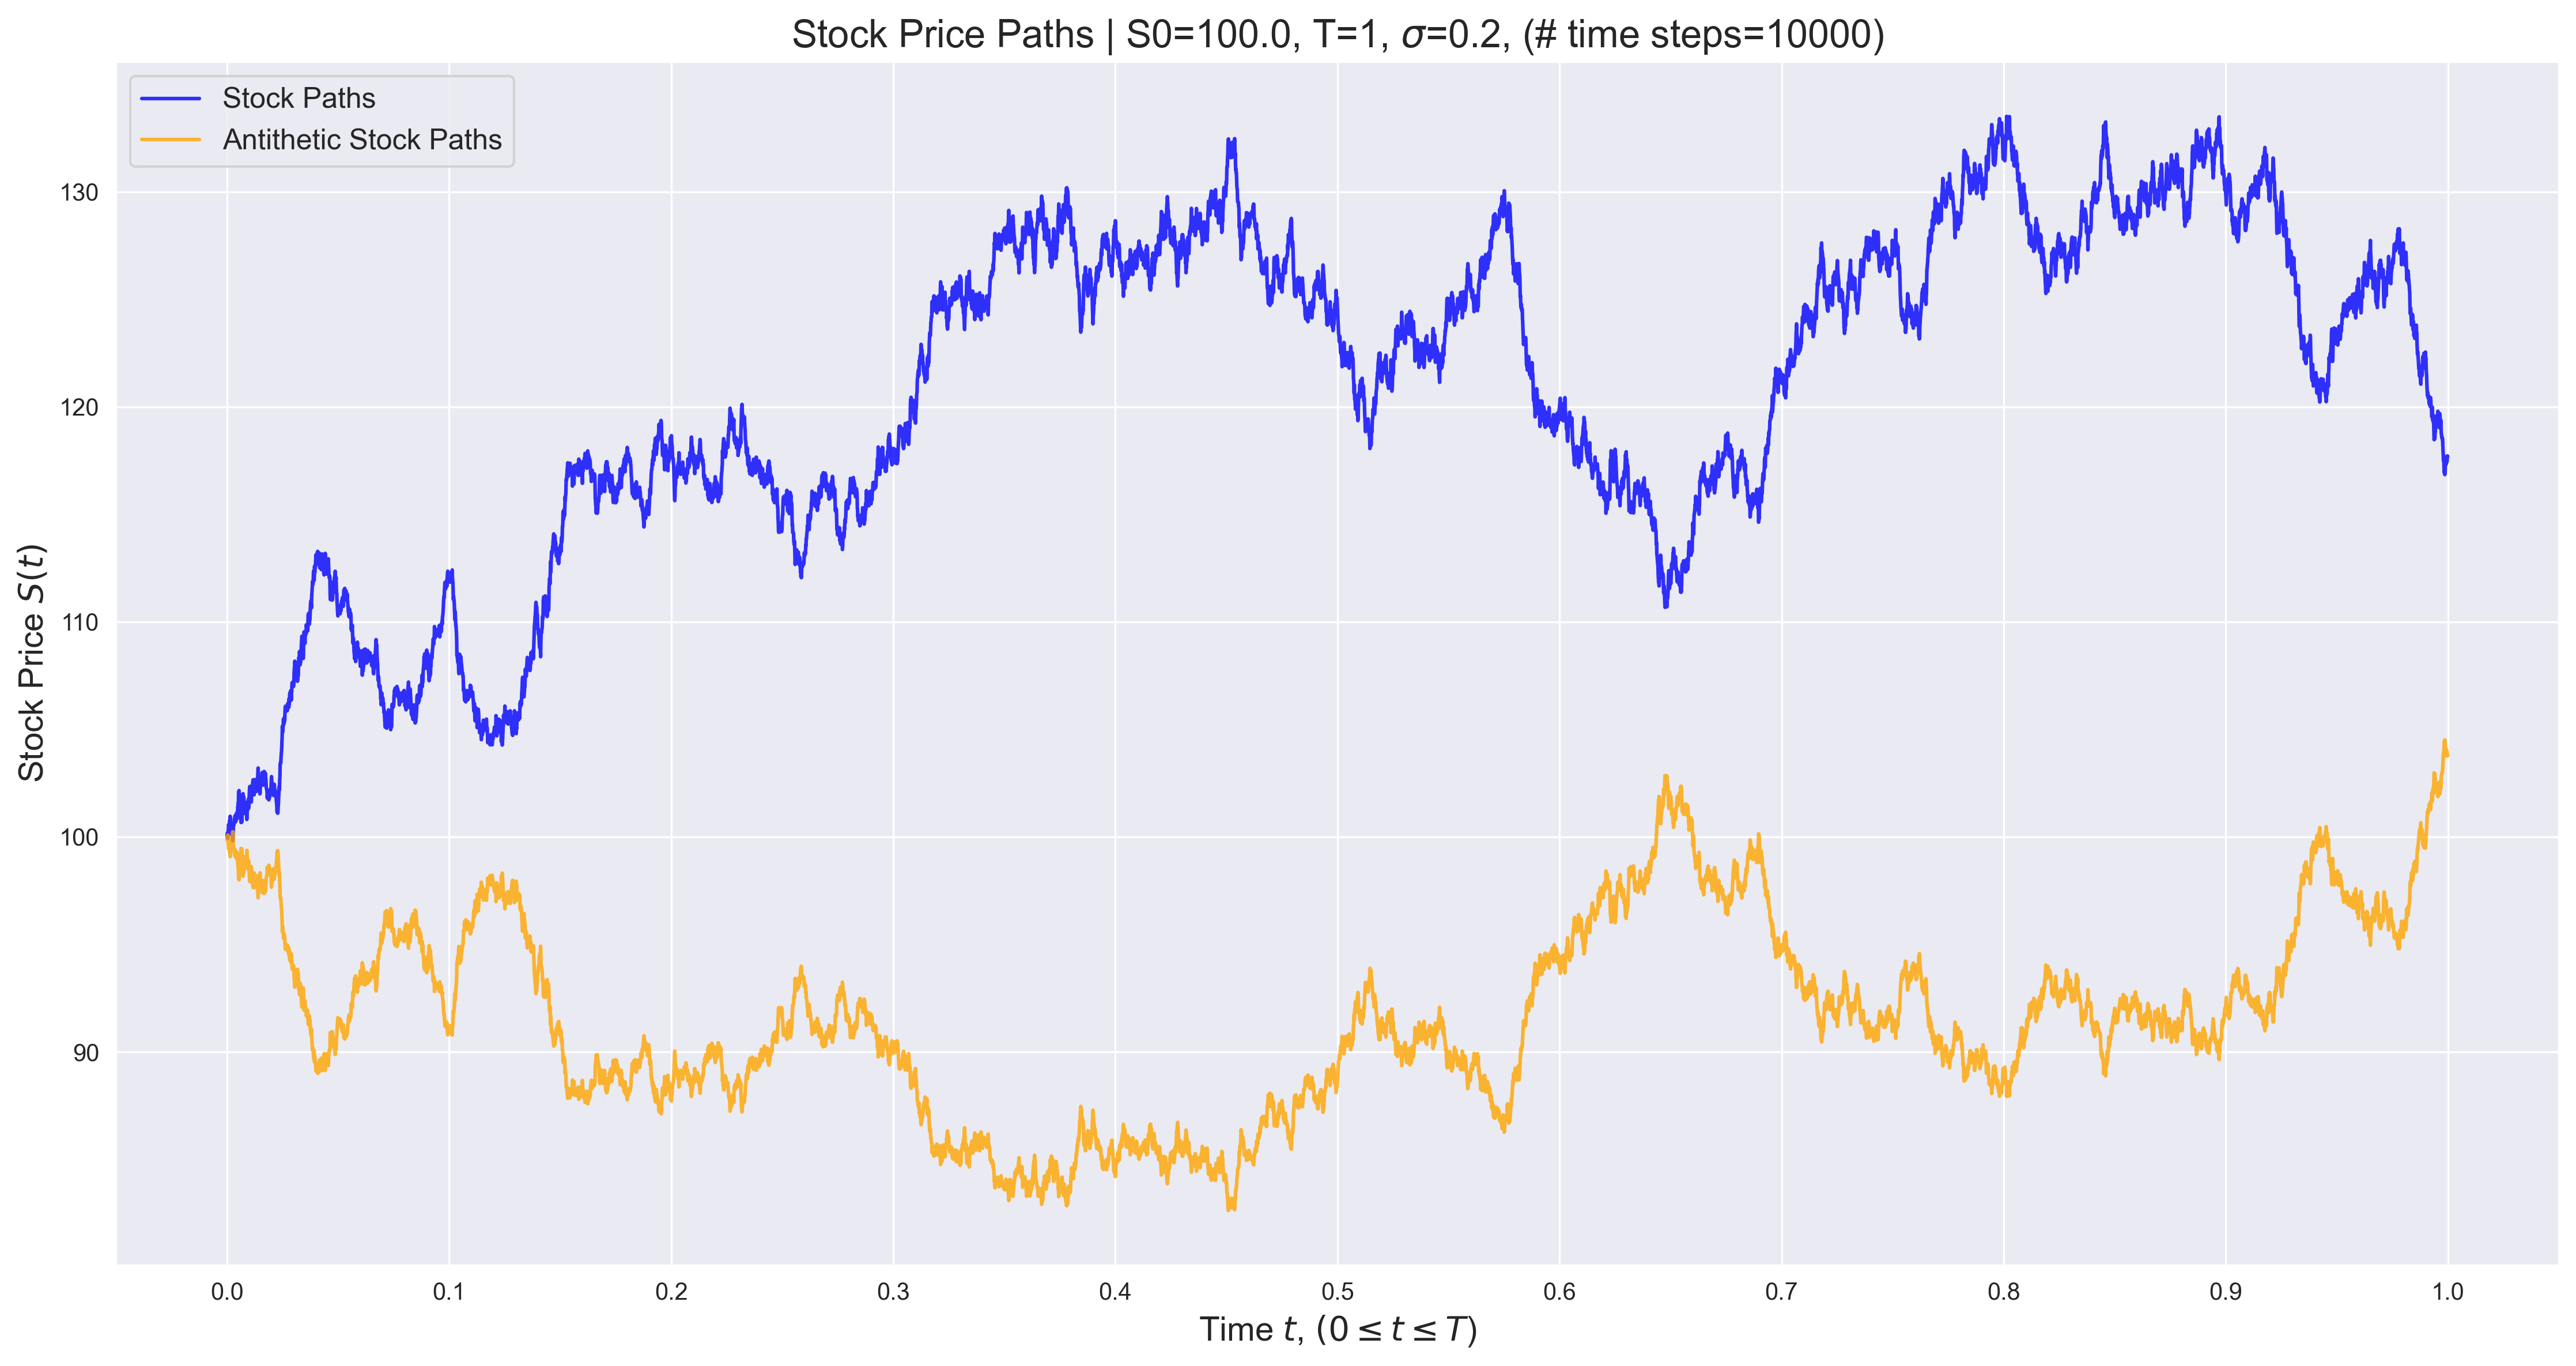
\includegraphics[width=\linewidth]{./figs/Trajectories.png}
    \caption{\it{Original and Antithetic path trajectories with $S(0) = 100$, $r = 0.1$, $\sigma = 0.2$}}
    \label{fig:figs}
\end{figure}

Denoting the original path payoff as \( \widehat{V}_i \) and the antithetic path payoff as \( \widehat{V}_i^{(a)} \), the new estimator for the expected payoff using antithetic variates (denoted by $\widehat{Y}_{AV}$) becomes
\[
\widehat{Y}_{AV} = \frac{1}{n} \sum_{i=1}^{n/2} \frac{ \widehat{V}_i + \widehat{V}_i^{(a)}}{2}.
\]

It is noted that each random sampling is used twice and only half of the original $n$ samples are required to be generated compared to the MCE. Denoting the MCE estimator as $\widehat{Y}_{MC}$, using antithetics reduce variance when
\[
    \text{Var} \left(\widehat{Y}_{AV}\right) = \text{Var} \left( \frac{1}{n} \sum_{i=1}^{n/2} \frac{ \widehat{V}_i + \widehat{V}_i^{(a)}}{2} \right) < \text{Var}\left(\frac{1}{n} \sum_{i=1}^{n}\hat{V}_i\right) = \text{Var}(\widehat{Y}_{MC});
\]
which can be reduced to the condition that
\[
    \text{Cov} \left(\widehat{V}_i, \widehat{V}_i^{(a)}\right) < 3 \text{Var} \left(\widehat{V}_i\right).
\]
Since the original and the mirrored trajectories have a low correlation, Horvath and Medvegyev states there is a substantial reduction in variance achieved through this approach \cite{nummethods}.

\subsubsection{Method of Control Variates}

The method of control variates reduces variance by incorporating a highly correlated variable (control variate) with a known expectation to the primary estimator. Let $Y$ be the appropriately chosen control variate for the arithmetic Asian option payoff \(\widehat{V}\).
The control variates estimator for \( \mathbb{E}[V(T)] \) (denoted by $\widehat{Y}_{CV}$) is then defined as
\[
\widehat{Y}_{CV} = \sum_{i=1}^n \frac{\widehat{V}_i + c Y_i}{n},
\]
where \(\widehat{V}_i\) and \(Y_i\) are the \(i\)-th simulated outcomes for the Asian payoff and control variate respectively and \(c\) is a constant. The value of \(c\) is chosen to minimize the variance of this estimator, given by \cite{nummethods}
\[
c^* = -\frac{\text{Cov}(\widehat{V}, Y)}{\text{Var}(Y)}.
\]
Then the variance of $\widehat{Y}_{CV}$ is given by
\begin{align*}
    \text{Var} \left(\widehat{Y}_{CV} \right) = \text{Var} \left( \sum_{i=1}^n \frac{\widehat{V}_i + c^* Y_i}{n} \right) & = \frac{\text{Var} \left( \widehat{V}_i \right) + (c^*)^2 \text{Var} \left( Y_i \right) + 2c^* \text{Cov}(\widehat{V}, Y)}{n} \\
    & = \frac{1}{n} \left( \text{Var}(\widehat{V}) - \frac{\text{Cov}(\widehat{V}, Y)^2}{\text{Var}(Y)} \right),
\end{align*}
which is always less than or equal to the variance of the original estimator \( \widehat{V} \). This demonstrates that the control variates method can yield substantial variance reduction if \( \widehat{V}\) and \(Y\) are sufficiently correlated.
A natural choice for the control variate \(Y\) in the context of arithmetic Asian option pricing is the payoff of the geometric-average Asian option \cite{kemna}. 
Geometric averages have closed-form solutions in the Black-Scholes framework, making their expected values easy to compute. Since the geometric average is also mathematically related to the arithmetic average, it serves as a suitable control variate that is closely correlated with the arithmetic Asian payoff \( \widehat{V}\). In practice, adding a “discretisation-adjusted” control variate also help correct for any approximation error arising due to the discrete time steps \( \{t_j\}_{j=0}^{m} \) used in simulations, further enhancing the accuracy \cite{nummethods}.

\section{Method}

\section{Result}

% \section{Summary}
% \input{Summary}

\newpage

\printbibliography

\end{document}

